\section{Testing}

Consider the following function, written in a C-like language, where \texttt{rand()} returns a pseudo-random (integer) number:
\begin{lstlisting}[style=C]
0: void foo() {
1:      int h, k;
2:      h = 0; 
3:      for (int i=0; i<10; i++) {
4:          if (h > rand()) 
5:              k++;
6:          else
7:              h++;
8:      } 
9:  }
\end{lstlisting}
\begin{enumerate}
    \item Build the Control Flow Graph of foo
    \item Derive all the reaching definitions at the entry and the exit of each block.
    \item According to the reaching definitions, derive all the UD chains and then def-use pairs for variables $h$ and $k$.
    \item According to the previous results, what are the potential problems of foo?
\end{enumerate}

\paragraph*{Solution}
\begin{enumerate}
    \item The Control Flow Graph of the function is derived from the code and is the following: 
        \begin{figure}[H]
            \centering
            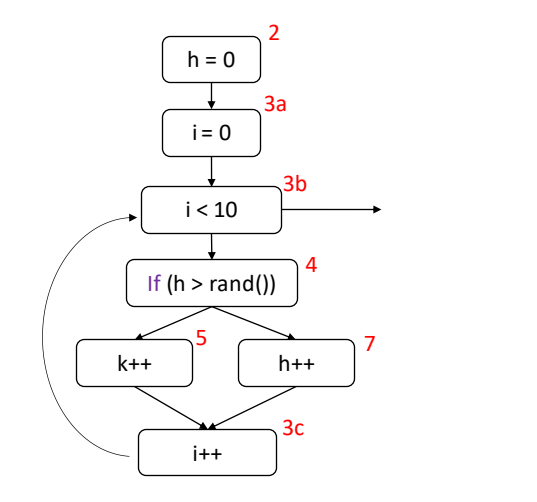
\includegraphics[width=0.5\linewidth]{images/cfg1.png}
        \end{figure}
    \item After executing once the loop we have the following reaching definitions: 
        \begin{figure}[H]
            \centering
            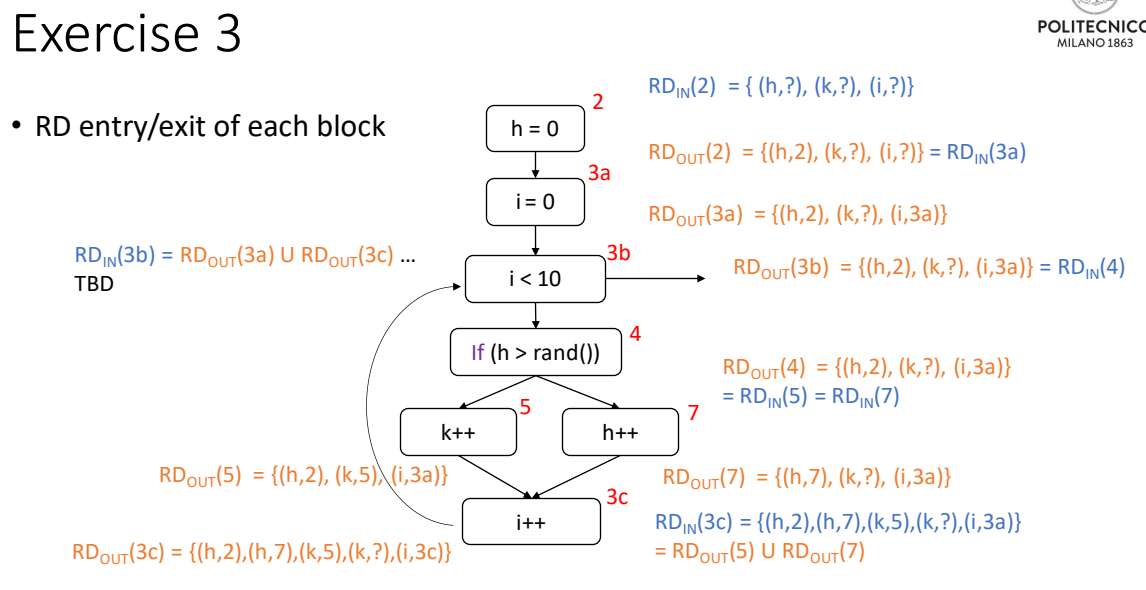
\includegraphics[width=0.5\linewidth]{images/rd.png}
        \end{figure}
        After the second iteration we have the following sets: 
        \begin{figure}[H]
            \centering
            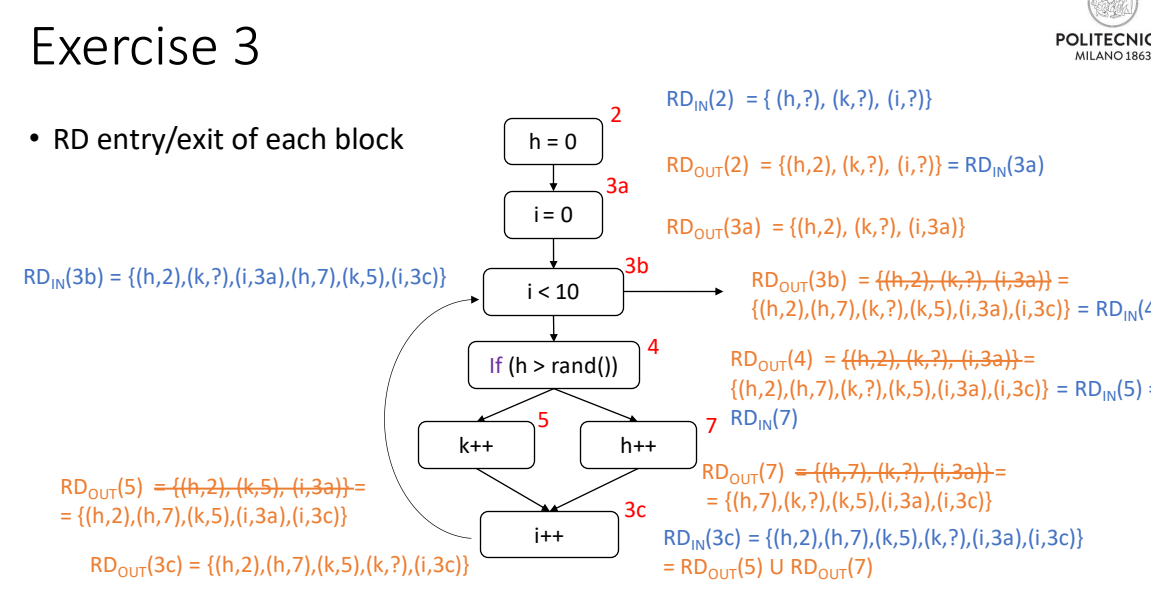
\includegraphics[width=0.5\linewidth]{images/rd1.png}
        \end{figure}
    \item The variable $h$ is defined in block four and in block seven. 
        In those two block the variable can be defined in different blocks: 
        \begin{itemize}
            \item $\text{UD}(h,4)=\{2,7\}$
            \item $\text{UD}(h,7)=\{2,7\}$
        \end{itemize}
        The variable $k$ is only used in block five and can be defined only in this block, as a result we have: 
        \begin{itemize}
            \item $\text{UD}(k,5)=\{5,?\}$
        \end{itemize}
        From the use-definition chains it is possible to define the def-use pairs as follows: 
        \begin{itemize}
            \item $h: \left\langle 2,4 \right\rangle, \left\langle 7,4\right\rangle, \left\langle 2,7\right\rangle, \left\langle 7,7\right\rangle$
            \item $k: \left\langle 5,5 \right\rangle, \left\langle ?,5\right\rangle$
        \end{itemize}
    \item We may have a problem with the variable $k$ since in one case it has a use without definition ($\left\langle ?,5\right\rangle$).
\end{enumerate}